%
% $RCSfile: communication.tex,v $
%
% Copyright (C) 2002-2008. Christian Heller.
%
% Permission is granted to copy, distribute and/or modify this document
% under the terms of the GNU Free Documentation License, Version 1.1 or
% any later version published by the Free Software Foundation; with no
% Invariant Sections, with no Front-Cover Texts and with no Back-Cover
% Texts. A copy of the license is included in the section entitled
% "GNU Free Documentation License".
%
% http://www.cybop.net
% - Cybernetics Oriented Programming -
%
% http://www.resmedicinae.org
% - Information in Medicine -
%
% Version: $Revision: 1.1 $ $Date: 2008-08-19 20:41:05 $ $Author: christian $
% Authors: Christian Heller <christian.heller@tuxtax.de>
%

\subsection{Communication}
\label{communication_heading}
\index{Communication}
\index{Information Processing}

As described in the previous sections, humans have sensoric and motoric organs
responsible for information input and output. In between input and output, the
information is processed by the brain that contains a specific abstract model
of the surrounding real world. The human brain consists of several regions
(section \ref{brain_regions_heading}), each being responsible for a special
task, such as the optical region for seeing or the cerebral cortex for actual
information processing which possibly leads to awareness. Depending on which
medium, organ and language is used, systems may communicate across different
channels.

%
% $RCSfile: transient.tex,v $
%
% Copyright (C) 2002-2008. Christian Heller.
%
% Permission is granted to copy, distribute and/or modify this document
% under the terms of the GNU Free Documentation License, Version 1.1 or
% any later version published by the Free Software Foundation; with no
% Invariant Sections, with no Front-Cover Texts and with no Back-Cover
% Texts. A copy of the license is included in the section entitled
% "GNU Free Documentation License".
%
% http://www.cybop.net
% - Cybernetics Oriented Programming -
%
% http://www.resmedicinae.org
% - Information in Medicine -
%
% Version: $Revision: 1.1 $ $Date: 2008-08-19 20:41:09 $ $Author: christian $
% Authors: Christian Heller <christian.heller@tuxtax.de>
%

\subsubsection{Transient}
\label{transient_heading}
\index{Transient Communication}
\index{Direct Communication}
\index{Assembler}
\index{Mapper}
\index{Translator}
\index{Signal Processing}

Valentin Turchin \cite{turchin} writes:

\begin{quote}
    Sensations are produced by our sense organs. Perceptions are formed and used
    within the brain. Conceptions are created by ourselves while we create new,
    linguistic, models of the world.
    The triad: Sensation, Perception, Conception seems close in meaning to Kant's
    usage of these terms. We leave it to the reader, though, to judge on it.
\end{quote}

The following example demonstrates a typical information processing procedure.
Its sequential flow is illustrated in figure \ref{handling_figure} which uses
technical names, instead of biological ones. These can be found again in the
explaining text, enclosed in parentheses. The terms \emph{Assembler} and
\emph{Mapper} are converted and merged into the term \emph{Translator}.

\begin{figure}[ht]
    \begin{center}
        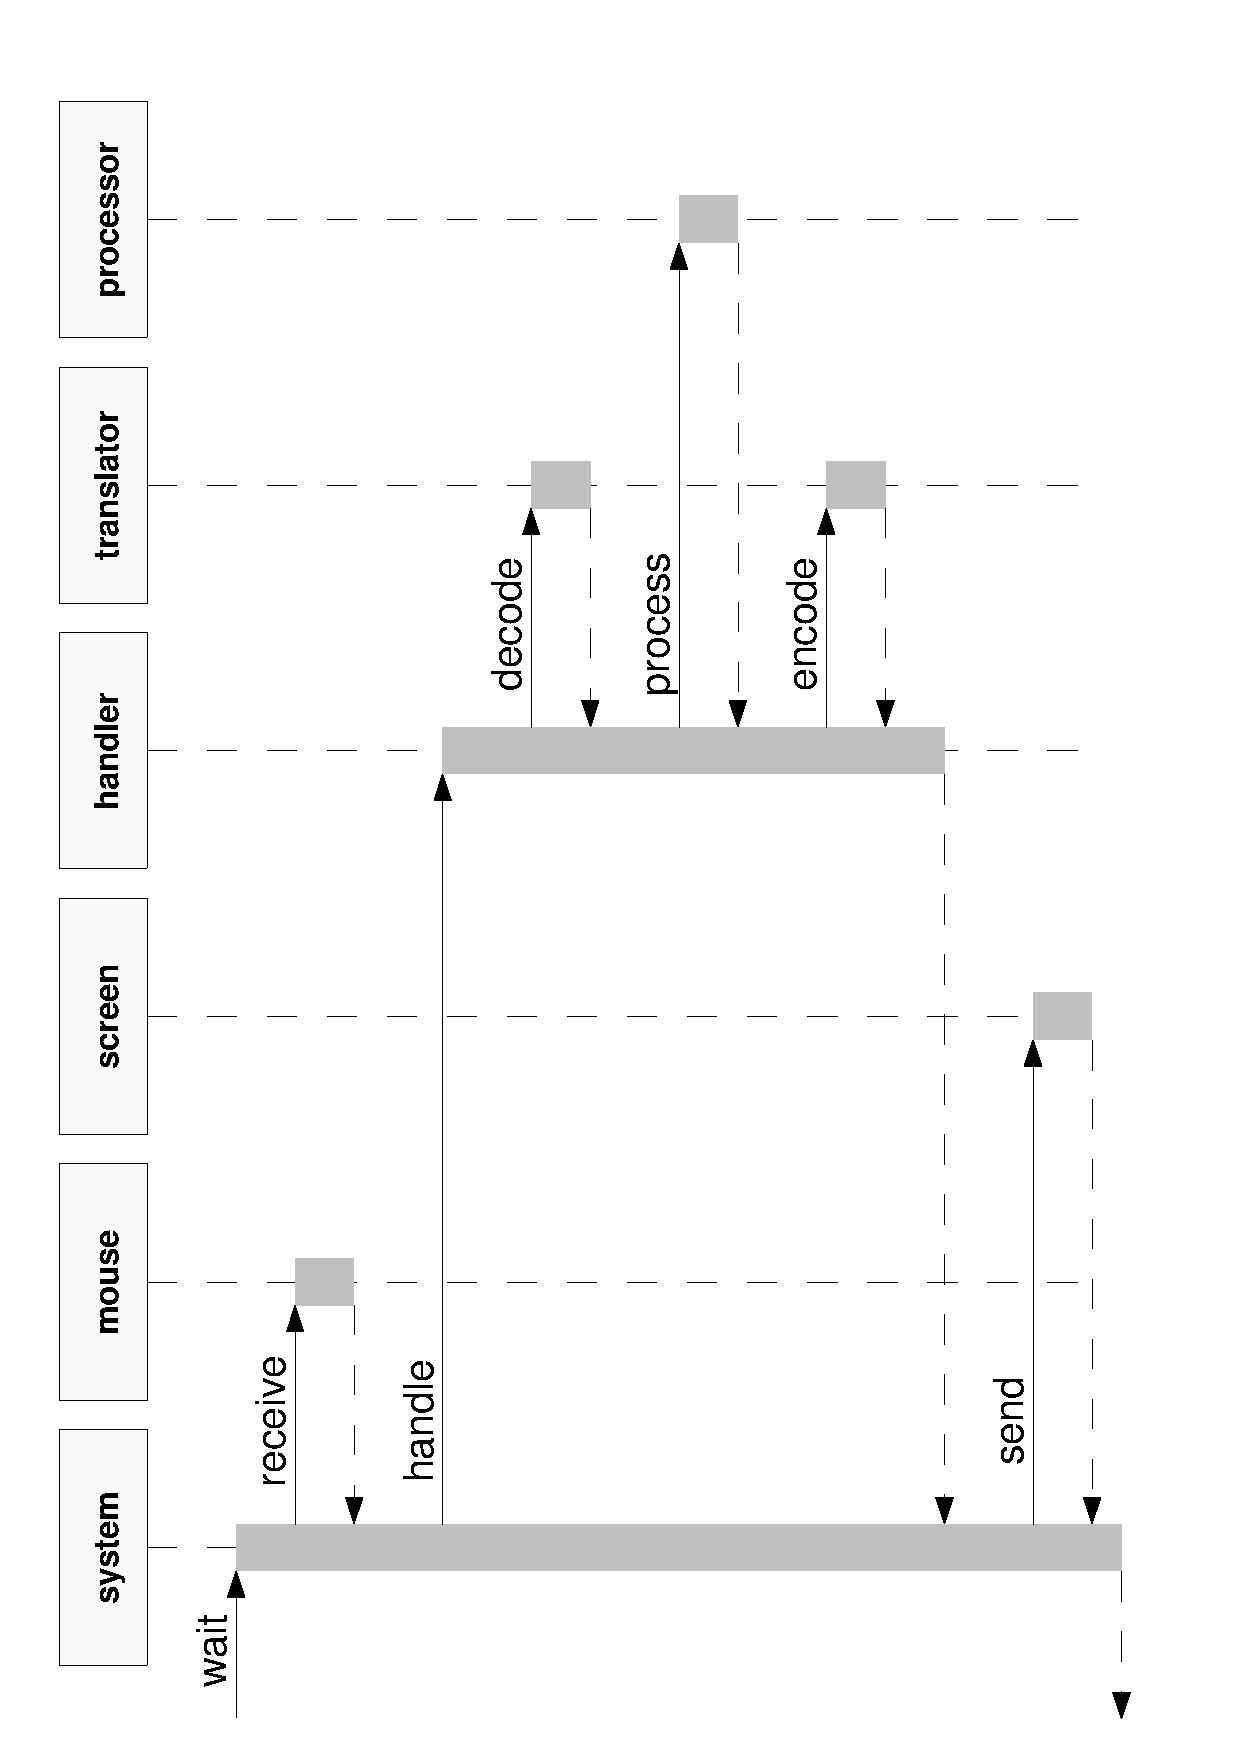
\includegraphics[scale=0.3,angle=-90]{graphic/handling.pdf}
        \caption{Signal Processing as UML Sequence Diagram}
        \label{handling_figure}
    \end{center}
\end{figure}

One human being (\emph{System}) wants to send a message to another. It decides
for an acoustical message (\emph{Signal}), formulates a sentence and talks. The
other human being, waiting for signals (\emph{wait}), receives the message
across its ear organ (\emph{Microphone}, \emph{Keyboard}, \emph{Mouse}). The
message is then forwarded to the receiver's brain (\emph{Handler}), where a
special region responsible for acoustics (\emph{Translator}) translates
(\emph{decode}) the data (\emph{Data Transfer Model}) contained in the message
and sorts them into the human's abstract model of the surrounding real world
(\emph{Domain Model}). Processing of the message happens in the cerebral cortex
of the brain (\emph{Processor}). If the addressed listener wants to send an
answer message (\emph{Signal}), it may do so by triggering a muscle reaction.
For this to happen, the motoric brain region (\emph{Translator}) needs to
translate (\emph{encode}) model data (\emph{Domain Model}) into a special
transfer model (\emph{User Interface Model}), for the answer. Finally, the
answer message (\emph{Signal}) will be sent as muscle action (data display on
\emph{Monitor}).

If a communication partner does not, or only partly receives a message, the
missing information is lost, unless the sender repeats it once more. The reason
is that the transport mediums (light, air) do not steadily contain the
information; the sent information is transient. Therefore, the whole process
described above can be called \emph{Transient Communication}.

%
% $RCSfile: persistent.tex,v $
%
% Copyright (C) 2002-2008. Christian Heller.
%
% Permission is granted to copy, distribute and/or modify this document
% under the terms of the GNU Free Documentation License, Version 1.1 or
% any later version published by the Free Software Foundation; with no
% Invariant Sections, with no Front-Cover Texts and with no Back-Cover
% Texts. A copy of the license is included in the section entitled
% "GNU Free Documentation License".
%
% http://www.cybop.net
% - Cybernetics Oriented Programming -
%
% http://www.resmedicinae.org
% - Information in Medicine -
%
% Version: $Revision: 1.1 $ $Date: 2008-08-19 20:41:08 $ $Author: christian $
% Authors: Christian Heller <christian.heller@tuxtax.de>
%

\subsubsection{Persistent}
\label{persistent_heading}
\index{Persistent Communication}
\index{Mediums for Knowledge Storage}
\index{Indirect Communication}
\index{Knowledge Carrier}
\index{Hard Disk Drive}
\index{HDD}
\index{Random Access Memory}
\index{RAM}

One great advantage of human beings is to be able to help each other, to
cooperate in order to reach a common aim, to form a society which is to fill
exactly these aims. Main tasks of a \emph{State} as one form of organisation of
society are: \emph{Security}, \emph{Education}, \emph{Social Welfare}. While
all of them depend upon \emph{Politics}, there is an additional factor playing
an increasingly important role: the \emph{Availability of Knowledge}. Knowledge
cannot only be exchanged between current citizens of earth; fortunately, it can
be forwarded over \emph{Generations}.

For this to become possible, mankind had to make use of different mediums for
external storage, such as: \emph{Rock Painting}, \emph{Stone Tablet},
\emph{Papyrus Roll}, \emph{Paper Book}, \emph{Chemical Film},
\emph{Electronic File}. It also had to invent technologies for the
dissemination of knowledge: \emph{Monks' copying by hand}, \emph{Library},
\emph{Printing}, \emph{Radio and TV}, \emph{Internet}. The following example
does therefore not deal with \emph{direct} inter-systems communication, but
rather its \emph{indirect} counterpart -- the interaction between a system and
mediums in its environment. Of course, that environment could be treated as
system, too; but for reasons of simplification it is not here.

One human being (\emph{System}) wants to send a message to another, which is
not near the same location, but at some remote place. The sender has to decide
for a persistent message, and to choose a non-transient medium to store that
message. He takes a piece of paper, writes down or paints some information and
finally sends that paper as letter by (snail) mail. Paper and letter act as
\emph{Knowledge Carriers}. The receiver may then perceive the message optically
and process it similarly to the transient communication explained in the
previous section.

Because the information in this example is permanently available and
reproducable from the external medium, communication processes of that kind may
be called \emph{Persistent Communication}. In computing, persistent information
can be stored in files on a \emph{Hard Disk Drive} (HDD), for example; data in
\emph{Random Access Memory} (RAM) or those sent over a network, on the other
hand, are transient.

The interpreter system introduced in chapter
\ref{cybernetics_oriented_interpreter_heading} is capable of using transient-
as well as persistent communication.

%
% $RCSfile: models.tex,v $
%
% Copyright (C) 2002-2008. Christian Heller.
%
% Permission is granted to copy, distribute and/or modify this document
% under the terms of the GNU Free Documentation License, Version 1.1 or
% any later version published by the Free Software Foundation; with no
% Invariant Sections, with no Front-Cover Texts and with no Back-Cover
% Texts. A copy of the license is included in the section entitled
% "GNU Free Documentation License".
%
% http://www.cybop.net
% - Cybernetics Oriented Programming -
%
% http://www.resmedicinae.org
% - Information in Medicine -
%
% Version: $Revision: 1.1 $ $Date: 2008-08-19 20:41:07 $ $Author: christian $
% Authors: Christian Heller <christian.heller@tuxtax.de>
%

\subsubsection{Models}
\label{models_heading}
\index{Communication Models}
\index{Agent as Social System}
\index{Communication Model by Shannon \& Weaver}
\index{Conversation Model by Osgood \& Schramm}
\index{Encoder}
\index{Decoder}
\index{Contents of Communication}
\index{Lasswell Formula}
\index{Sender (Who) as Communication Element}
\index{Receiver (Whom) as Communication Element}
\index{Message (What) as Communication Element}
\index{Language (Channel) as Communication Element}
\index{Result (Effect) as Communication Element}

Section \ref{agent_oriented_programming_heading} described a (software)
\emph{Agent} as \emph{social} system communicating with other agents, including
human beings \cite[p. 330]{sowa}. Various communication process models were
contributed by the \emph{Social Sciences}. Buesch \cite{buesch} describes a
\emph{Mathematical Communication Model} by Shannon \& Weaver (figure
\ref{shannon_figure}) that shows very well the presence of two translators:
\emph{Encoder} and \emph{Decoder}.

\begin{figure}[ht]
    \begin{center}
        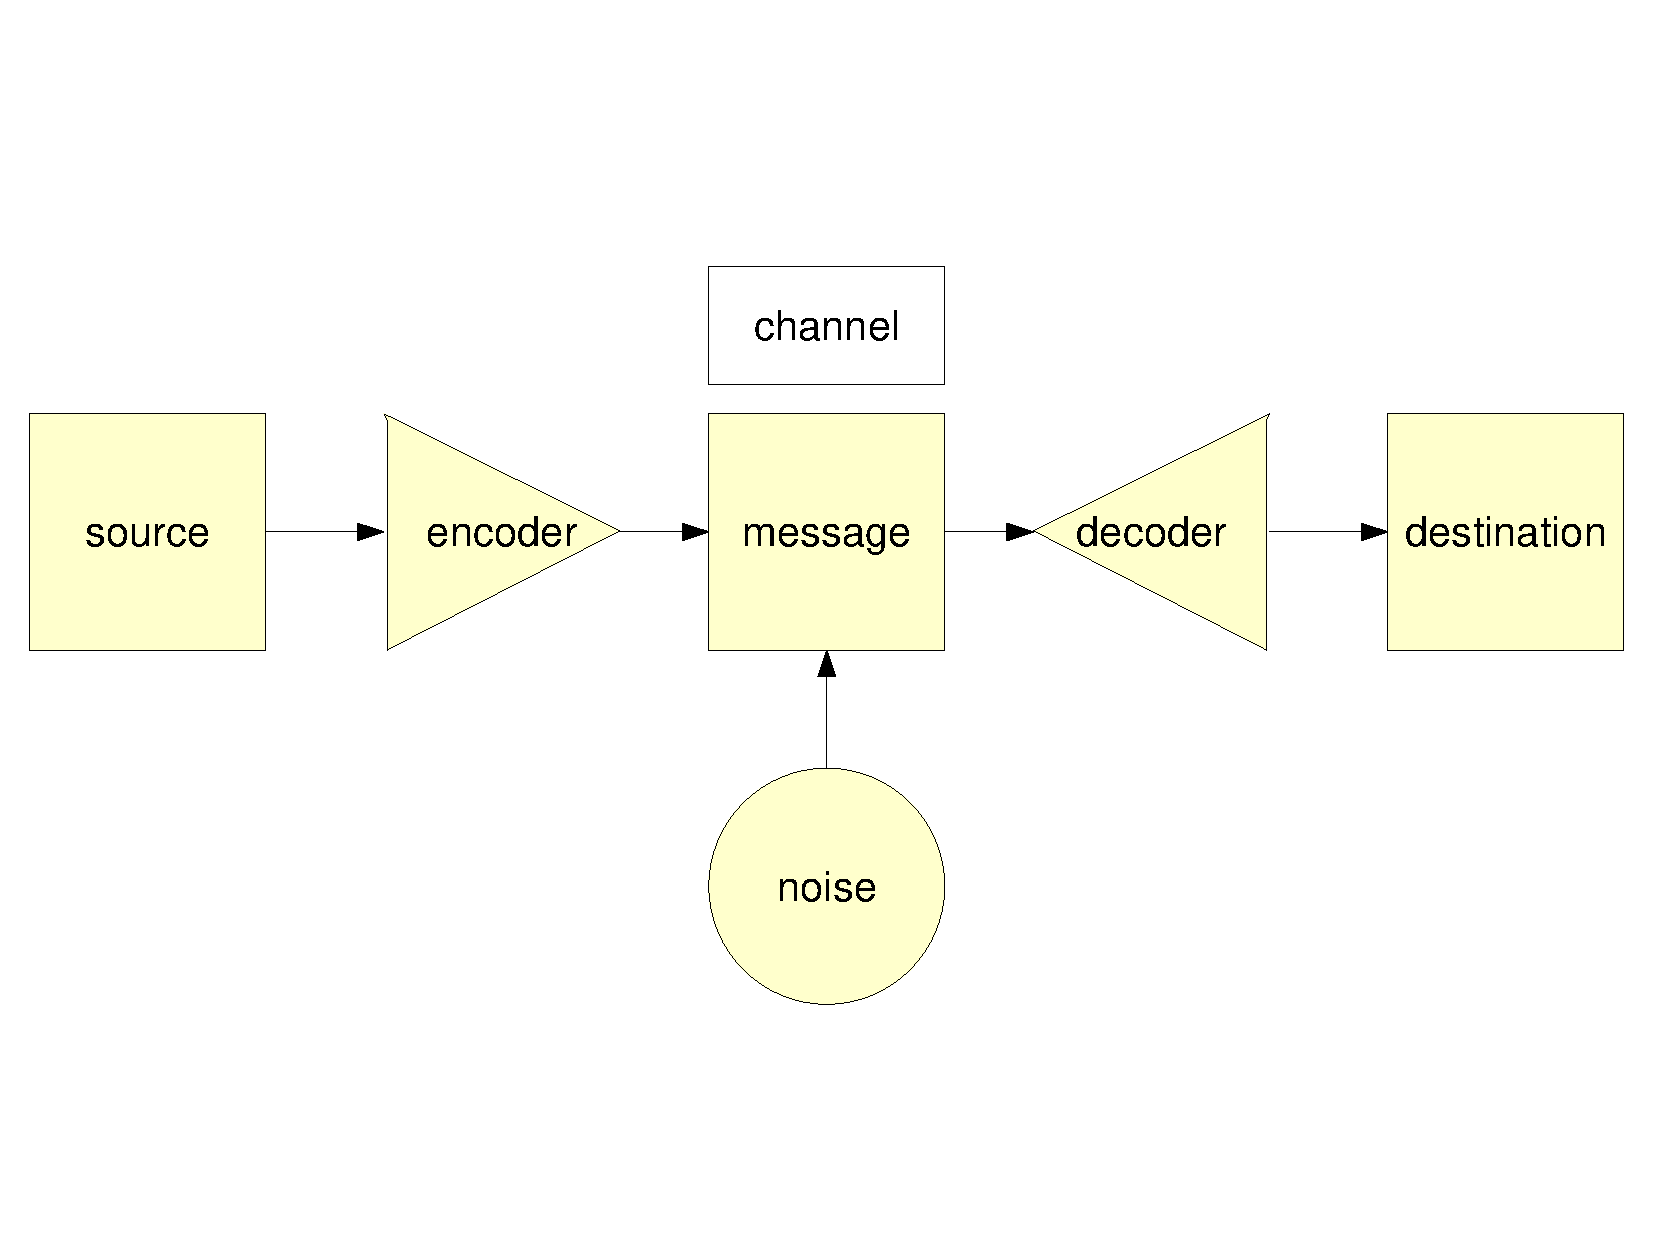
\includegraphics[scale=0.3,angle=-90]{graphic/shannon.pdf}
        \caption{Mathematical Communication Model by Shannon \& Weaver \cite{shannon}}
        \label{shannon_figure}
    \end{center}
\end{figure}

The \emph{Conversation Model} of Osgood \& Schramm (figure \ref{osgood_figure})
extends the communication model to a circular process of \emph{Question} and
\emph{Answer}, of \emph{Sending} and \emph{Receiving}. It shows more clearly,
that \emph{every} system, in order to communicate both ways, needs to own an
\emph{encoding} as well as a \emph{decoding} translator. The interpreter system
introduced in chapter \ref{cybernetics_oriented_interpreter_heading} contains
both kinds of translators.

\begin{figure}[ht]
    \begin{center}
        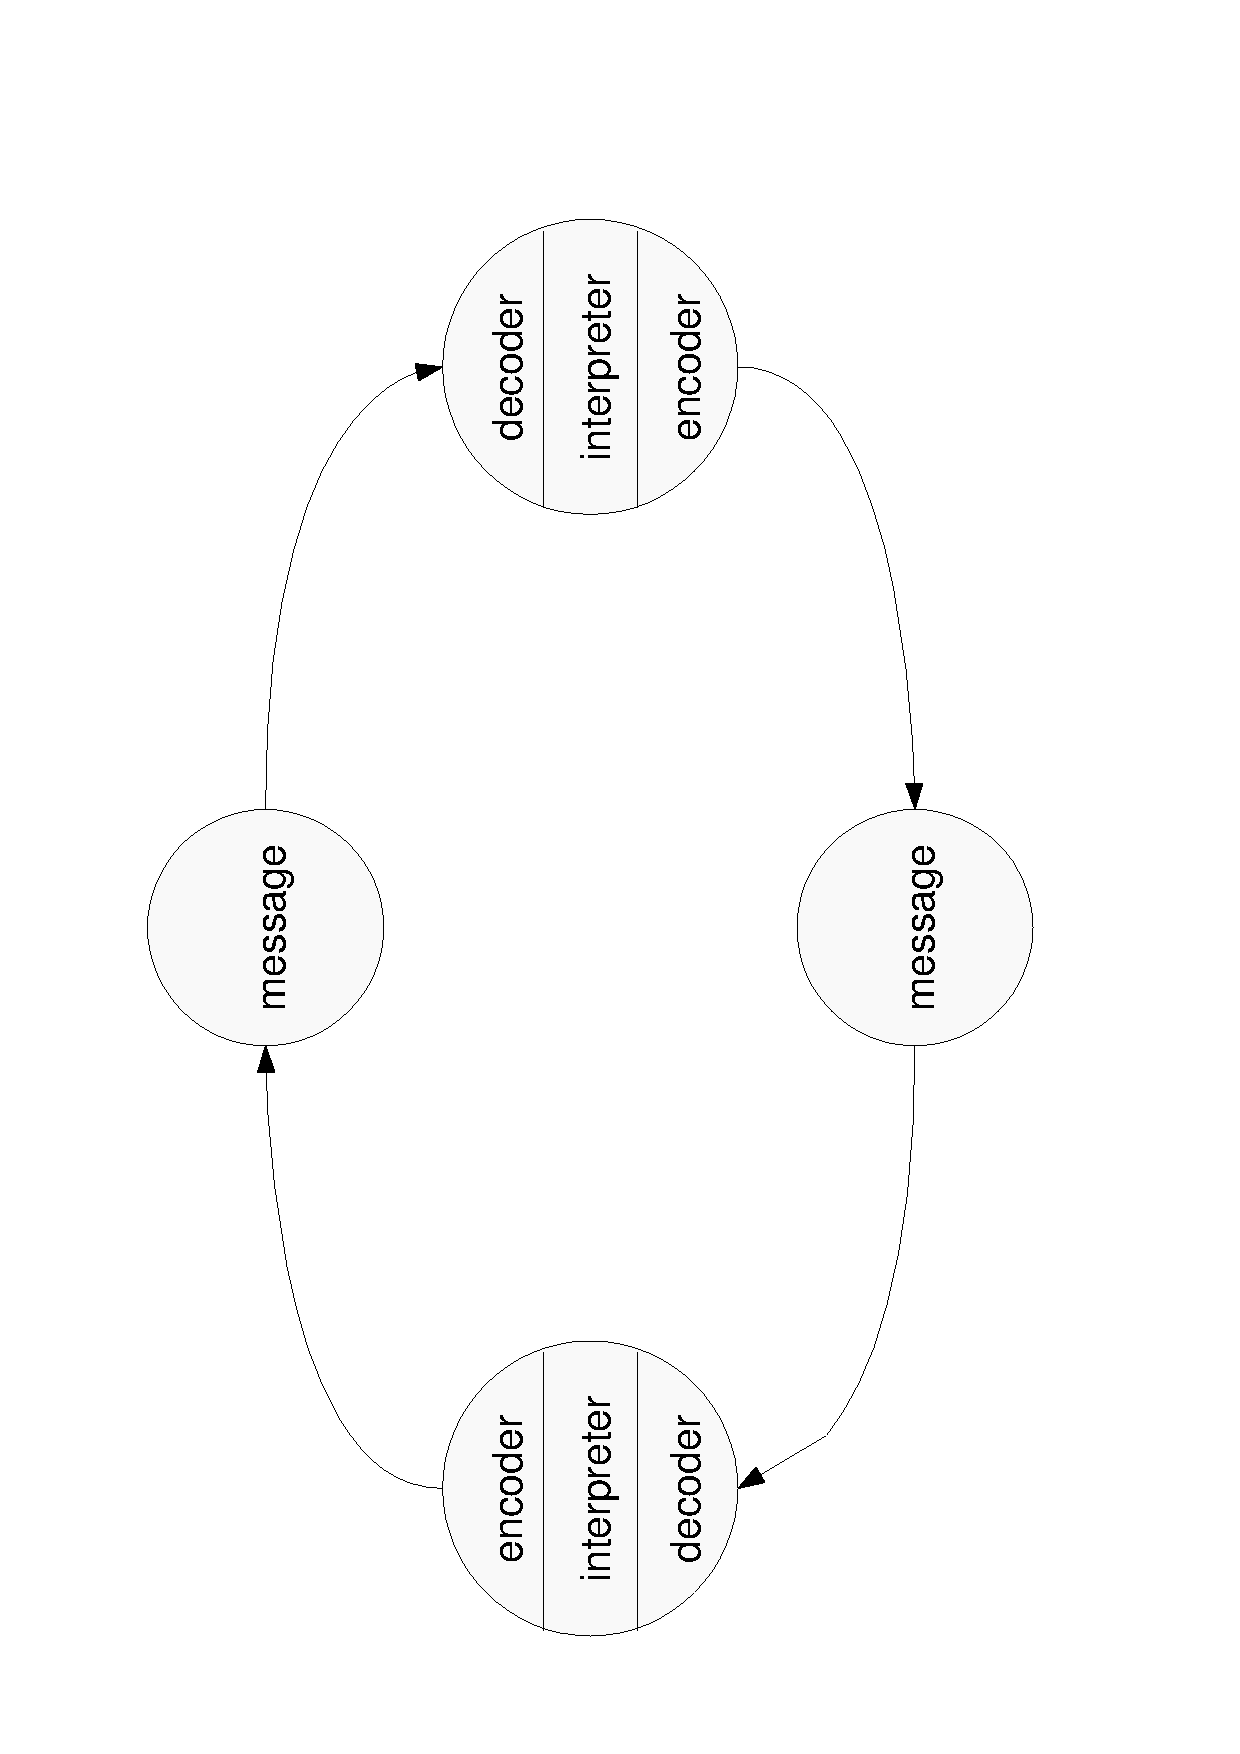
\includegraphics[scale=0.3,angle=-90]{graphic/osgood.pdf}
        \caption{Conversation Model by Osgood \& Schramm \cite{osgood}}
        \label{osgood_figure}
    \end{center}
\end{figure}

The \emph{Contents of Communication} is described by the
\emph{Lasswell Formula} (figure \ref{lasswell_figure}). After it, communication
consists of the five elements: \emph{Sender} (Who) and \emph{Receiver} (Whom),
\emph{Message} (What), \emph{Language} (Channel) and \emph{Result} (Effect).
The first four of these will be considered in the specification of the
knowledge modelling language introduced in chapter
\ref{cybernetics_oriented_language_heading}. The effects a communication has
(fifth element) are not a prerequisite for that communication to happen and
thus not interesting in the context of its technical realisation, as
investigated later in this work.

\begin{figure}[ht]
    \begin{center}
        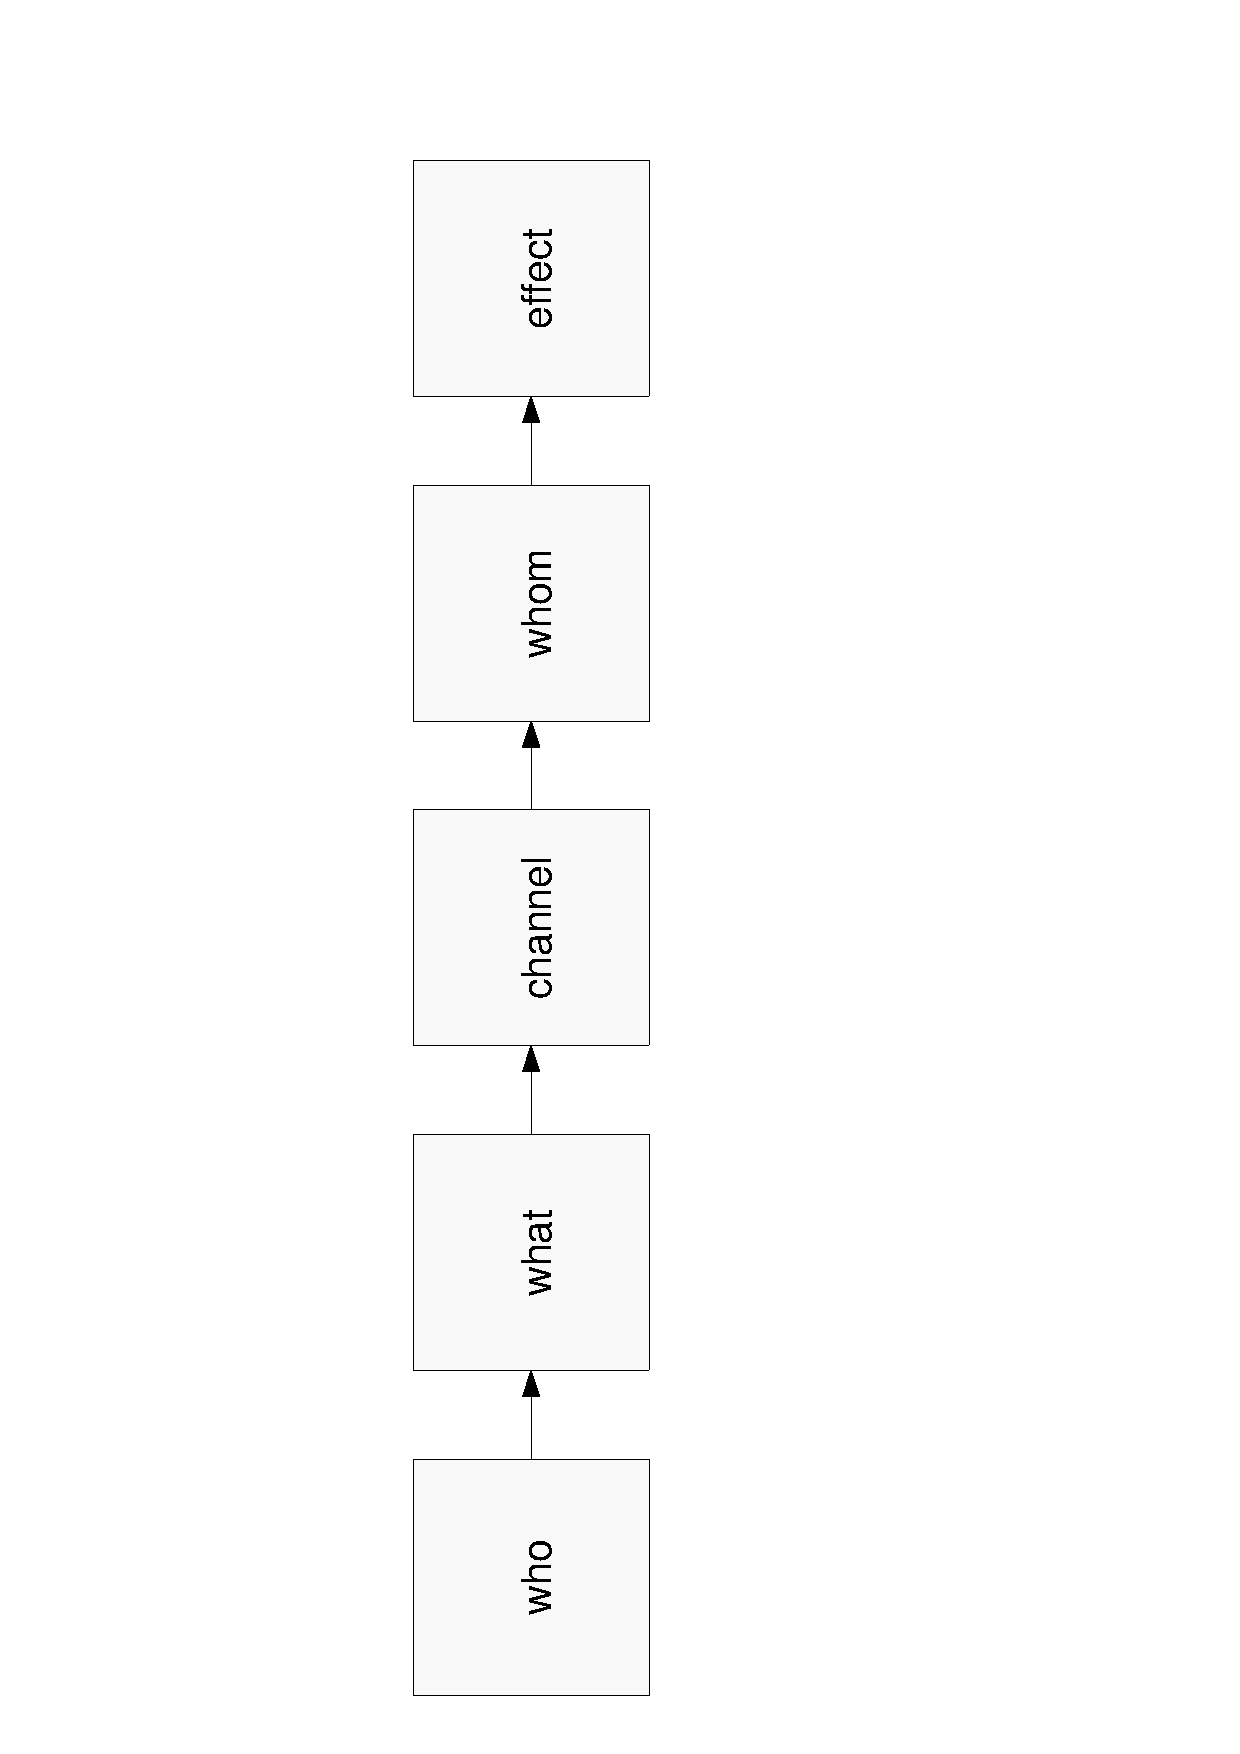
\includegraphics[scale=0.3,angle=-90]{graphic/lasswell.pdf}
        \caption{Contents of Communication (Lasswell Formula) \cite{lasswell}}
        \label{lasswell_figure}
    \end{center}
\end{figure}

